\newpage
\chapter{Methods and Methodology}
\begin{quote}
"The power of an image is that it embodies the complexity of what we see, feel and think but cannot literally describe in words." Tufnell and Crickmay, p.(2004)
\end{quote}

\newpage

\begin{figure}[htbp]
\begin{center}
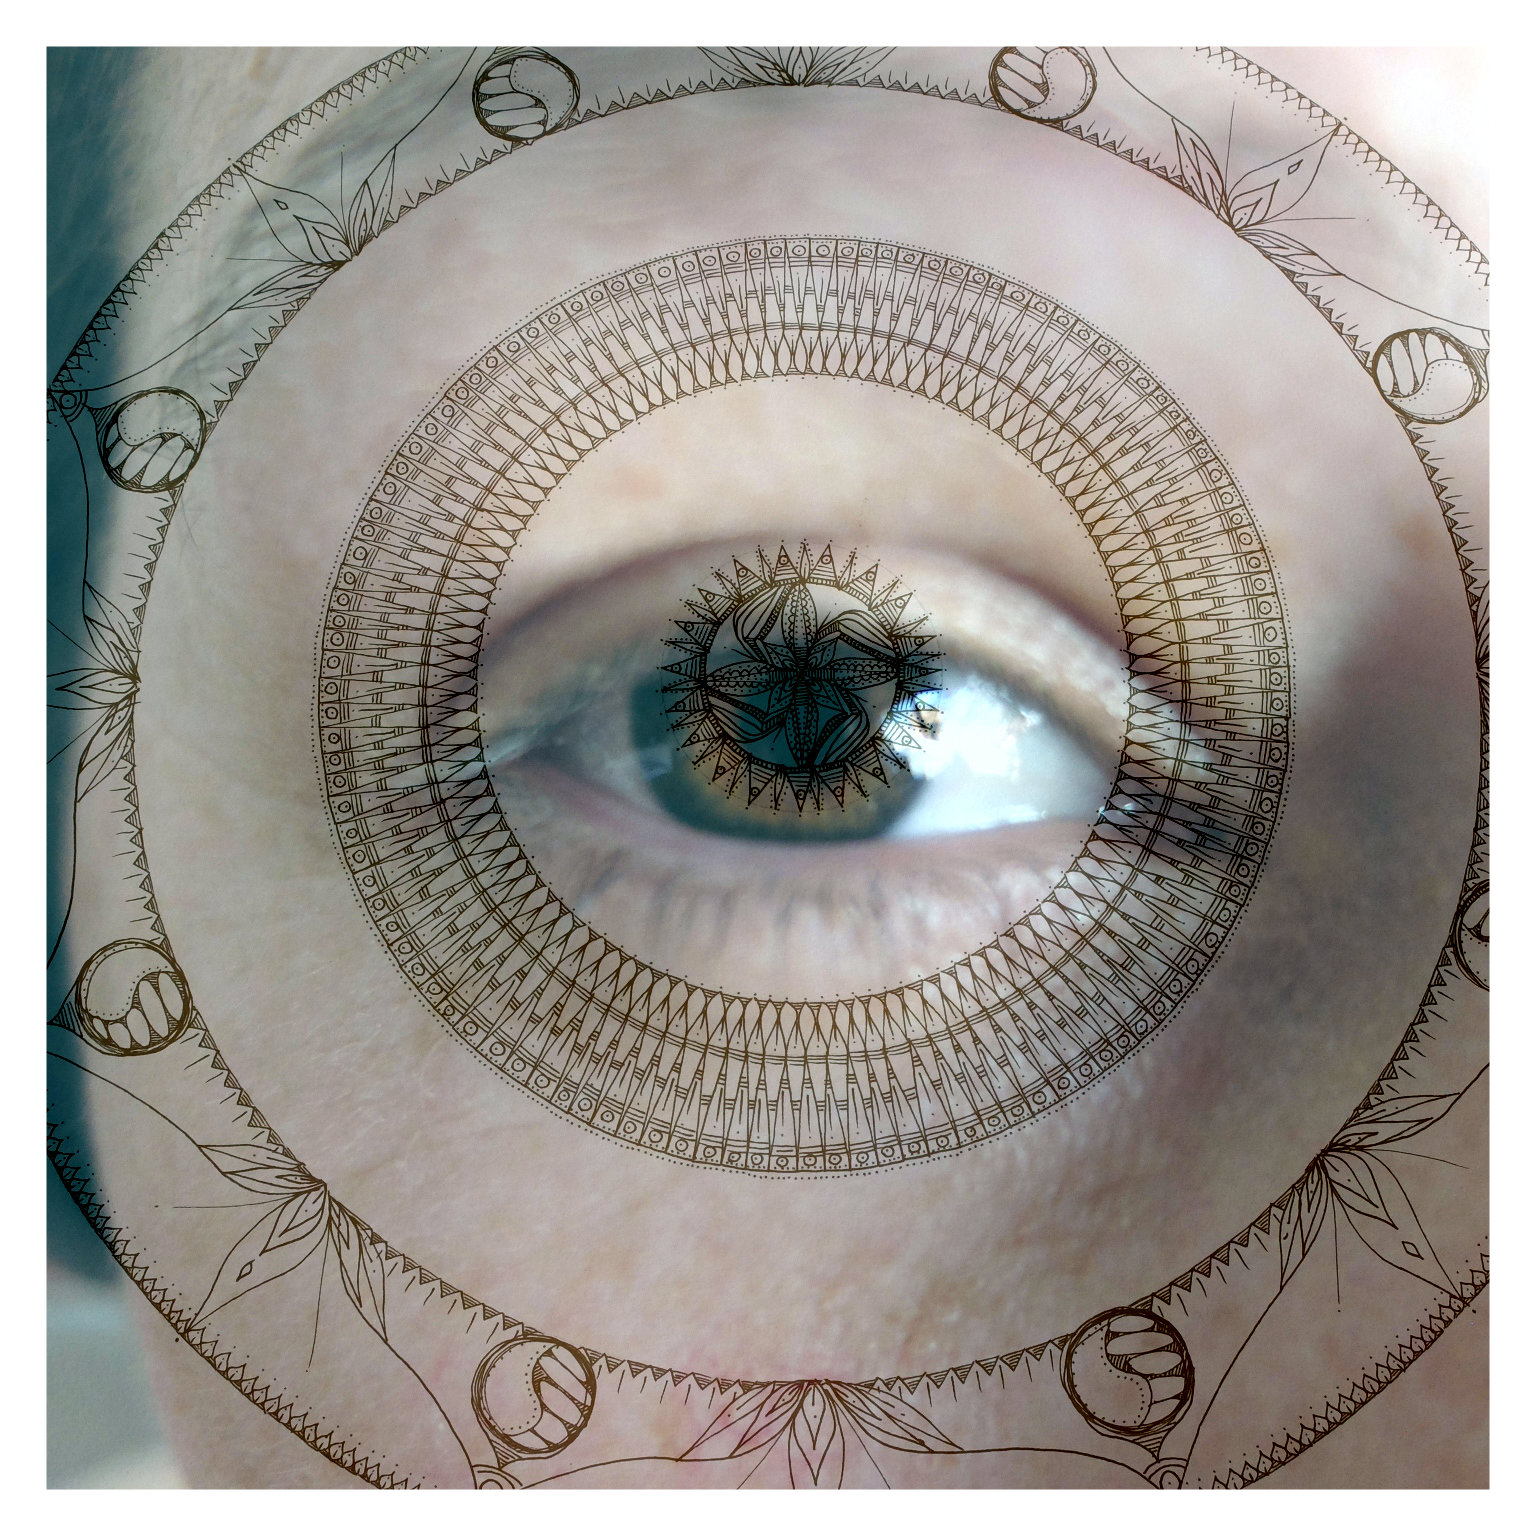
\includegraphics[scale=.3]{../eps/Double_exposure_eye_mandala.eps}
\caption{Double exposure eye mandala}
\label{label}
\end{center}
\end{figure}
%FIGURE 1-DOUBLE EXPOSURE WITH MY EYE AND MANDALA

\newpage

As you have already read, my research inquiry starts with my passion for drawing mandalas and I inquire into the journey of what I have come to know through this process. 
\begin{enumerate}
\item I began with an introduction and background information why I am inquiring in mandalas.  
\item I now move into my methods and methodology. As well as my procedures, paradigm alignment and my values I hold within my thesis. 
\item 
Following my methods and methodology I have predominately worked with my own data. I have drawn 6 mandalas and I have described the following: the making process of each mandala, key words, dialogue which happened within the process as well as pictures which illustrates the process of creations. You will find the following 6 mandalas in the following chapters. After the 6 mandalas, I have further explored and amplified them. 
\item 
Next, I have also included others experiences of drawing mandalas and their perspectives in my inquiry.
\item 
I then present the key words and essence words which are derived both my participants and from my own data. 
\item 
Then, by focusing on the process of drawing a mandala within a therapeutic context and its relevance and benefits. I provide with a creative synthesis and practical example to conclude.
Update 
\end{enumerate}

\section{Methodology}

My research is qualitative and circular. The notion that a circle has no beginning nor end is similar to the concept of us continuously evolving, shifting and transforming as beings. Throughout my process of drawing within mandalas I have continuously shifted and evolved within myself. 

I consider mandalas to have the capacity to delve into my unconscious parts of myself and cut through any pretence. Words do not come naturally for me, but images do. When I use my imaginative visualizations and images I create, I step beyond my analytical restrictions and become liberated to bring together my vocabulary and imagery and thus make sense of the experience I am exploring. Consequently, when attending to these key images, I feel they connect me with my pre-reflexive knowing and help to form my new knowing. 

The word mandala comes from the Sanskrit word which denotes essence and circle. Mandalas are ancient and have been used throughout history within many different cultures and religions. Thus, indigenous cultures used mandalas as symbols for healing and transformation. However, research into the healing aspects of drawing mandalas in the psychology field are rare. 

\section{Methods}


I have chosen an Arts as Inquiry approach which uses the arts first-hand in the inquiry to conduct meaning making from the arts itself. This inquiry uses many different modalities such as: drawing, movement, photography, sound, play, poetry and tattooing.

I have also used The MIECAT form of Inquiry, which has no predetermined or fixed methodology. Instead the process allows an emergent integrative flow of knowing and ways of being in the companioning process.  

The MIECAT form of Inquiry strengthens the feeling-emotion-thinking-valuing connectedness and attends to the here and now with a subjective and descriptive manner. The inquiry is placed around making meaning of the lived experience and what we have come to know. Dr Dan Siegel states: 

\begin{quotation}
"We need to empower people and say it is not what happened to you, it is how you make sense of what happened to you. He also said that the research also shows, that you are likely to repeat that, wether it's abuse, neglect or emotional distance if you have not made sense of those experiences." 
\end{quotation}

As Lett says 
\begin{quote}"since so much experience is not encoded verbally, and the explication of stored meanings is usually more complex than verbal skills alone can convey." (p, 1992) 
\end{quote}

When we combine multimodalities with dialoguing and experiencing pre-reflective and less conscious states, we bring together a variety of languages of the visual nature, pre-reflective knowings and intuition in combination with our cognitive language. Thus, by using a variety of modes we gain access to our own wisdoms, as well as having a better understanding of ourselves and the world around us. 

The procedure I used in my quite conversations within mandalas was an Arts as Inquiry. I was open to the awareness of my body and I endeavoured to stay present to my felt sensing. I bracketed in and out my thoughts. I also had a sense of moving in and out of collapsed time. In this collapsed time, I embark into my memories and simultaneously experienced the feelings of the present and the past. 

Hypnotically, I move the piece of paper around whilst I draw. I drift away with my emotions and feelings and at times my thoughts were in a vacuum of nothingness. I simply draw the same line over and over and, as a result, I become so immersed in the drawing process that I forgot to write key words as I had initially intended. 

Creating a mandala, I start by drawing a large circle with the compass, then keeping the sharp end in the paper, I move the pencil end of the compass, to make a few more circles within the larger circle.  I work from inside out and I intuitively make lines, dots and shapes. I never use measurements or sketch out the design. As McNiff says:
\begin{quote} "I can never know in advance what will appear, because I discover what is going on inside me through the process of painting." (p,1998). 
\end{quote}

I feel that any process of creativity is the same when it comes to discovering what is inside us. The only element in my mandalas which is not drawn freehand is the circles drawn with a pencils on the compass. These circles are erased and function as lines on the page to guide me.  


\section{Procedures}


\begin{figure}[htbp]
\begin{center}
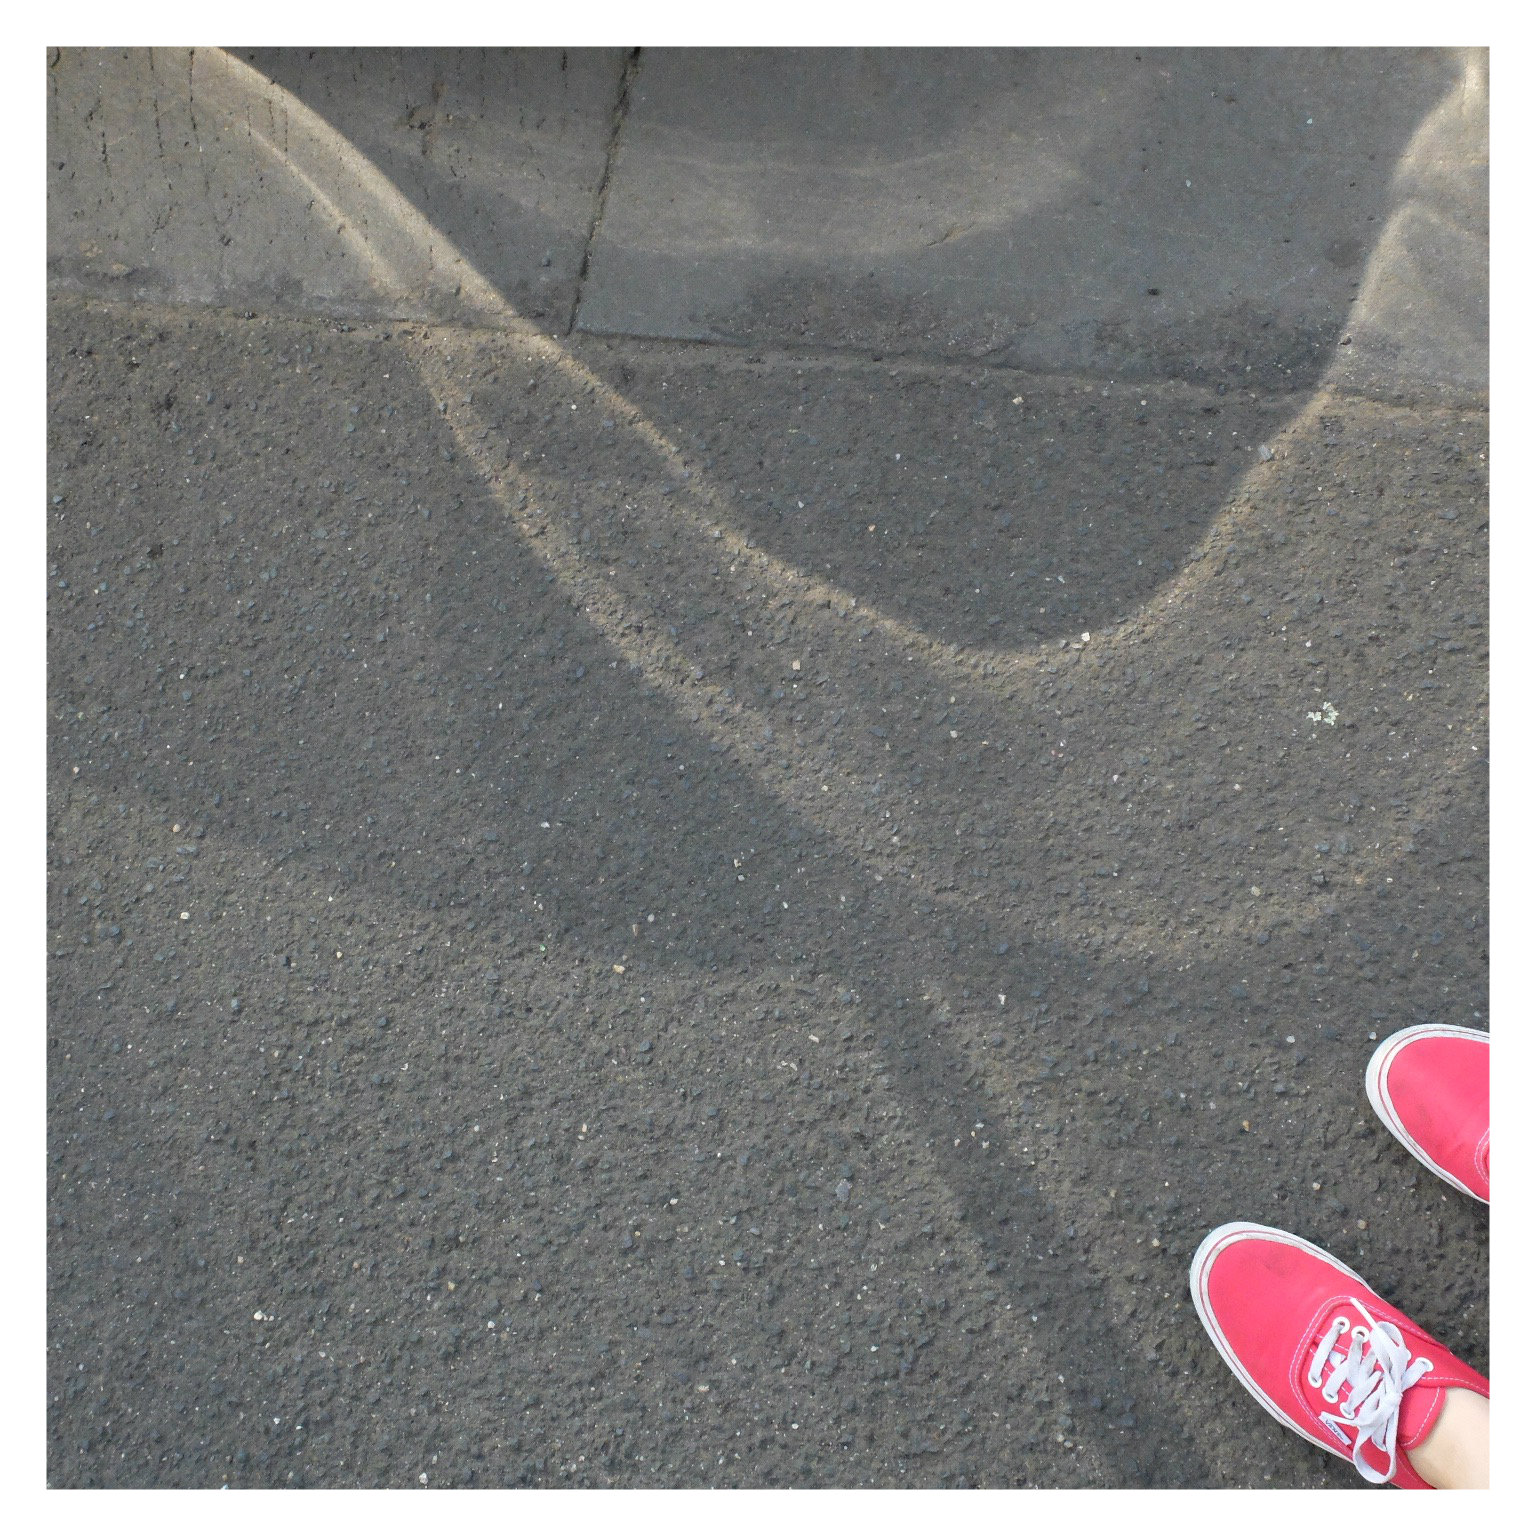
\includegraphics[scale=.3]{../eps/Stepping_into.eps} 
\caption{The procedures I stepped into}
\label{label}
\end{center}
\end{figure}

%FIGURE 2-THE PROCEDURES I STEPPED INTO


The procedures I used in creating and making my own mandalas are the following:
\begin{itemize}
\item Attending to the present moment
\end{itemize}

\begin{itemize}
\item Accessing lived experiencing 
\end{itemize}

\begin{itemize}
\item Finding emergent expression through mandala form
\end{itemize}

\begin{itemize}
\item Starting off with my emotional state, engaging with art making and noticing the changes and shifts within myself
\end{itemize}

\begin{itemize}
\item Remained with a descriptive attitude 
\end{itemize}

\begin{itemize}
\item Key words
\end{itemize}


After drawing the 6 mandalas, I remained attuned and aware to the slightest changes within me. I sat with all my personal data to deliberately amplify its content to come up with the themes and topics which arose. I also kept generating more data as the year went on through keeping a mandala diary. 
Additionally, I added these procedures to the mix: 

\begin{itemize}
\item Reduction to what is important 
\end{itemize}

\begin{itemize}
\item Essence key words/images
\end{itemize}

\begin{itemize}
\item Clustering key words
\end{itemize}

\begin{itemize}
\item Designing and getting a tattoo
\end{itemize}

\begin{itemize}
\item  'I' poems- An 'I'poem is the process where a piece of text is underlined only with the I and the accompanying word. This highlights associative stream of consciousness carried by the first person and how the writer speaks about themselves. (Gilligan, spencer, Weinberg, Bertsch 2006). On the listening guide- A voice-centred relational methods, Gilligan, spencer, Weinberg, Bertsch 2006, Sage publications
\end{itemize}

Within the process of my own work and companioning others, the following procedures are adapted to the context and situations. They are as follows:
\begin{itemize}
\item Description- where one is descriptive and states what can be seen in basic terms 
\end{itemize}

\begin{itemize}
\item ISR- (Intersubjective response)- a response offered to the other
\end{itemize}

\begin{itemize}
\item  Clustering- grouping together images and words which fit together* Representations- can be expressed through using many art modality art forms
\end{itemize}

\begin{itemize}
\item Reduction- reducing large images and text to key words and images 
\end{itemize}

\begin{itemize}
\item Bracketing- where we bracket in and out our own thoughts, as well as being aware of our own feelings and sensations only sharing with the other what is helpful and appropriate
\end{itemize}

\begin{itemize}
\item Accessing to experiencing- We can sense or be aware of our less conscious states along with conscious parts through accessing our experiences through connecting to our emotions, thoughts, sensations, imagery, memories, smell, visualisations, bodily sensations and feelings
\end{itemize}

\section {Maps}
The following are mind maps of the steps and procedures I took:
%maps



\section{Paradigm alignment}

\begin{figure}[htbp]
\begin{center}
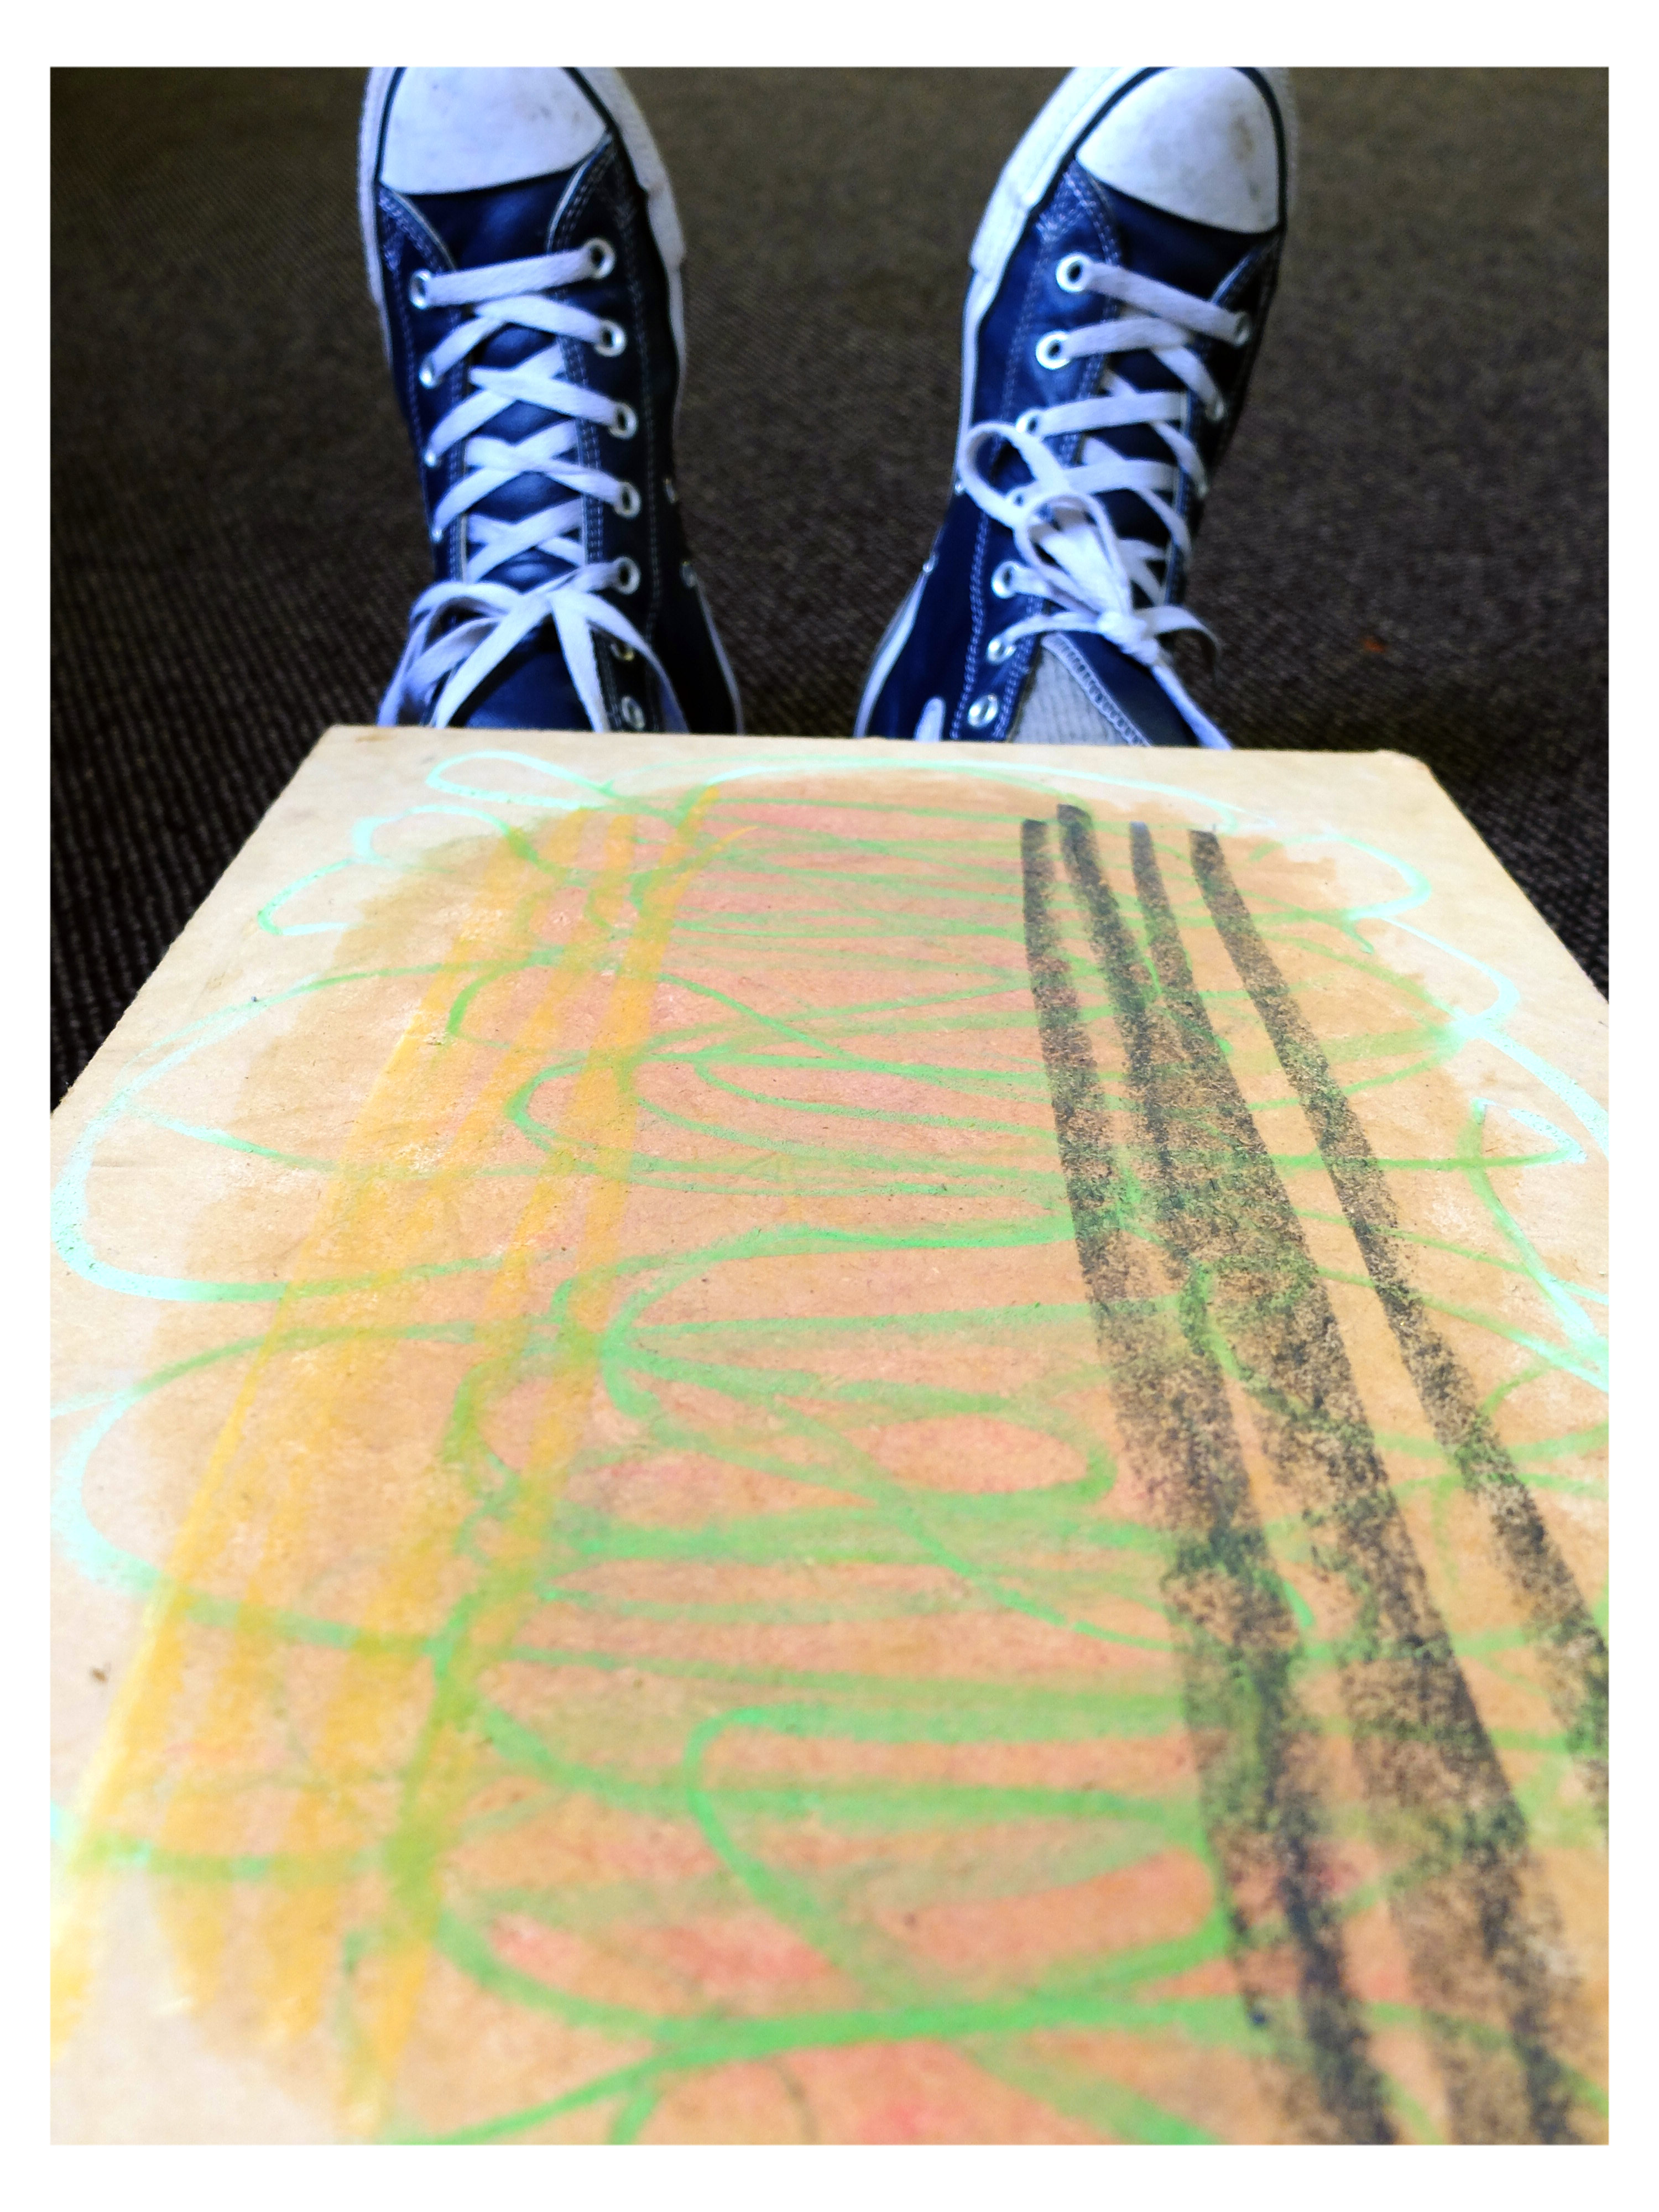
\includegraphics[scale=.1]{../eps/My_allignment_and_shoes.eps} 
\caption{My alignment and shoes}
\label{label}
\end{center}
\end{figure}
\newpage

%FIGURE 3- MY ALIGNMENT AND SHOES


Things are not as fixed as I once thought, hence I have come to know that I sit in a Post-modern paradigm. We are relational beings and we constantly change and evolve. We are in an integrative flow and companion and co-construct every moment. Therefore, we all make the choice to participate and inquire into each other and our relationships around us. I feel we need to take the time to re-connect both with others and ourselves because of this constant evolution of our lives. I wrote this in reflection:


\begin {centering}As they change, we change\newline 
As we change, they change\newline 
So, do we accept or do we fight it?\newline 
Do we ignore it or adapt?\newline 
Is it hidden or do we see it?\newline 
We aspire to relate and connect\newline 
And as we change and they change\newline 
We make the choice\newline 
To transform together or apart\newline 
\end {centering} 



\begin{figure}[htbp]
\begin{center}
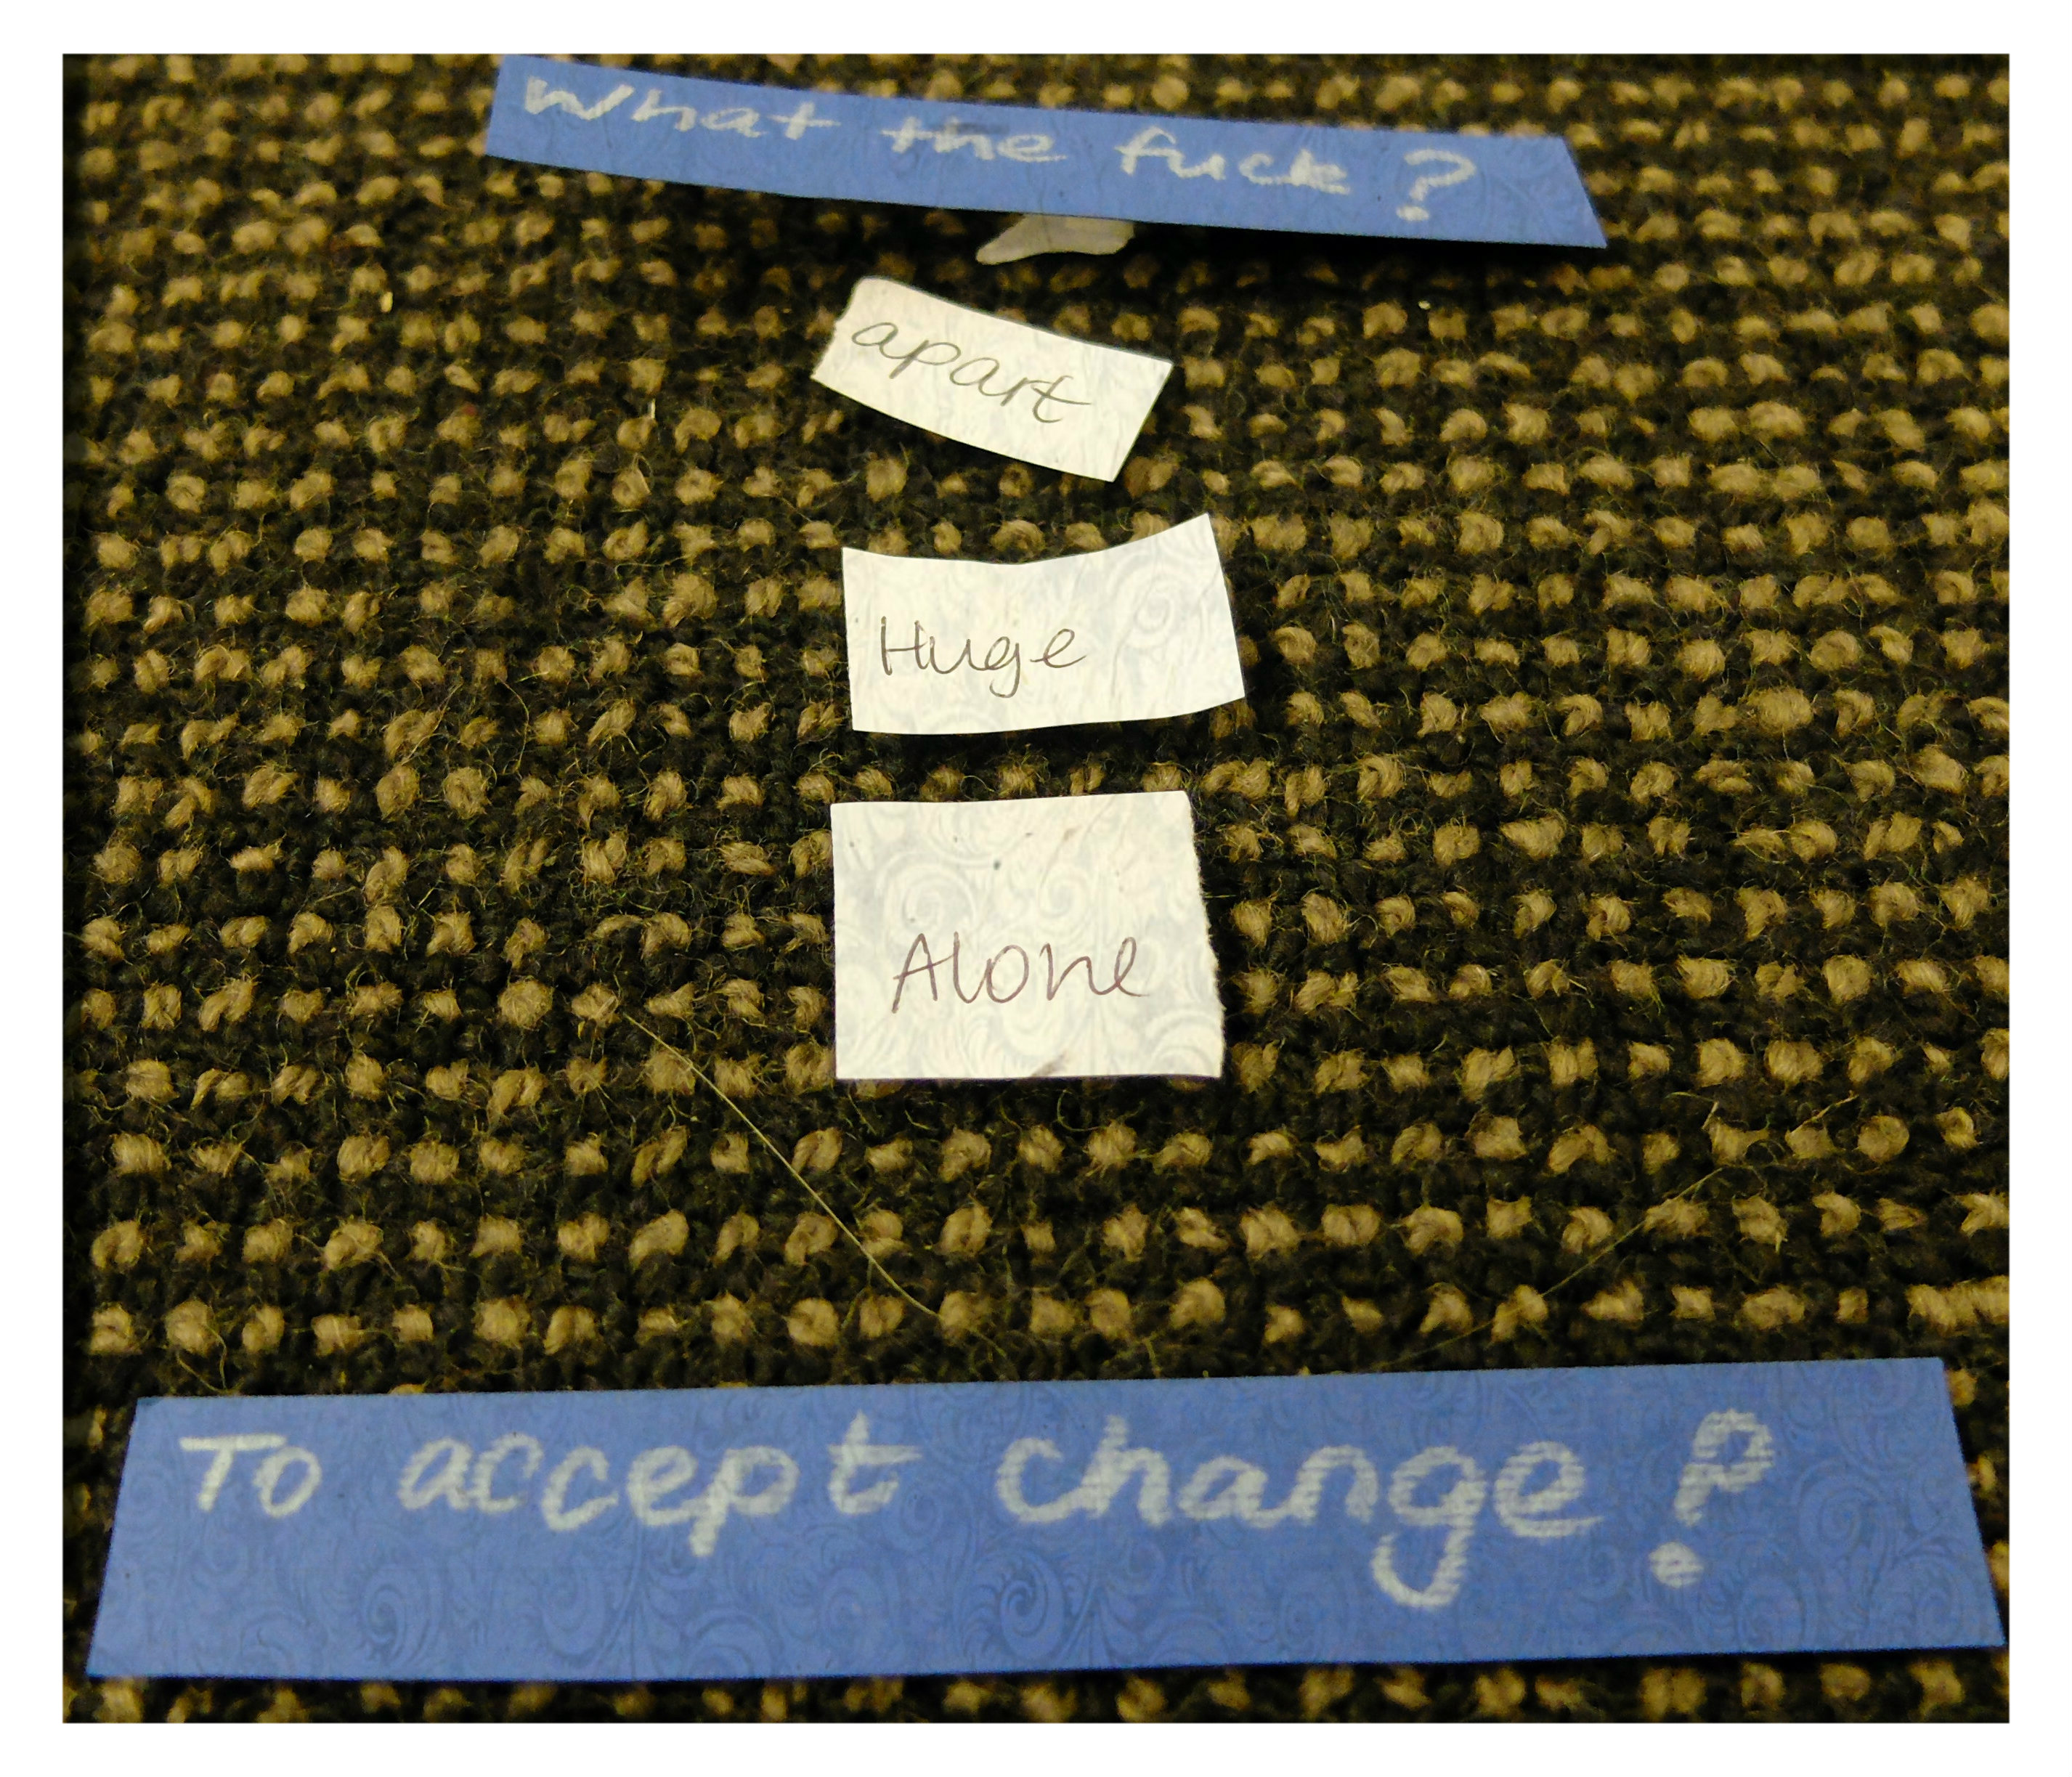
\includegraphics[scale=.1]{../eps/What_the_fuck.eps} 
\caption{What the fuck?}
\label{label}
\end{center}
\end{figure}
\newpage
%FIGURE 4- WHAT THE FUCK?


